\subsection{CapTap}
\begin{figure}[h]
\centering
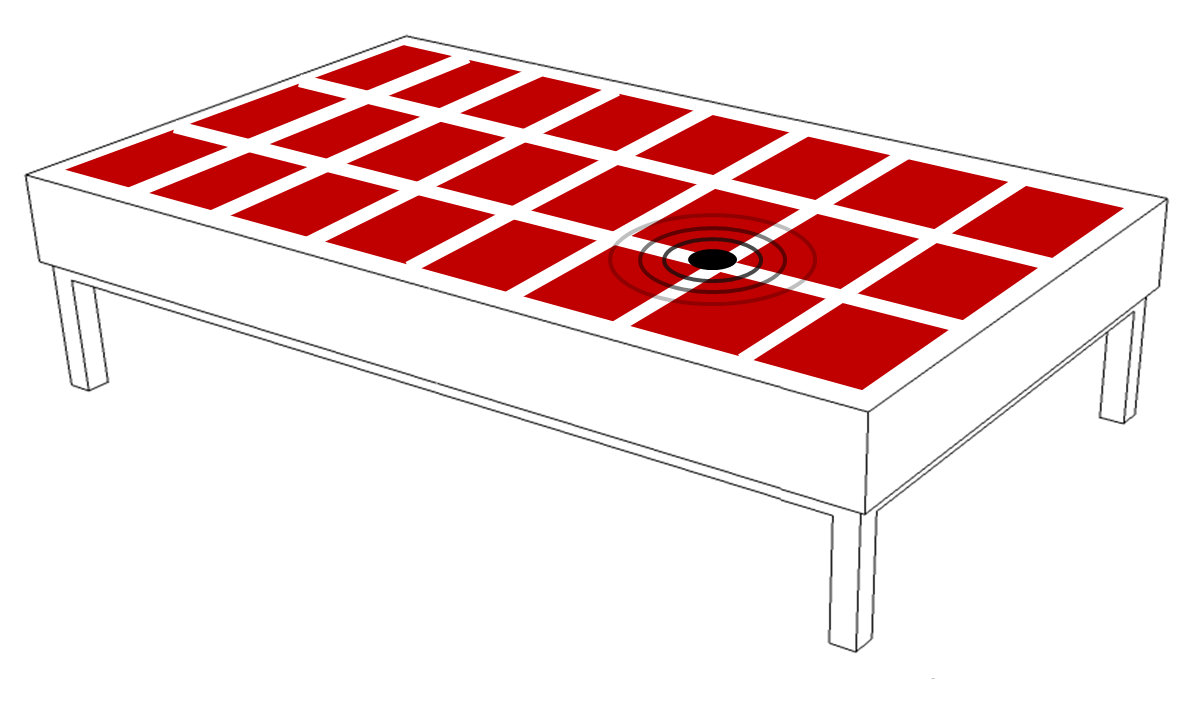
\includegraphics[width=0.7\textwidth]{images/captap_v2}
\caption{CapTap sketch - 24 electrodes placed under table surface}
\label{fig:captap_sketch}
\end{figure}
%Figure 33 CapTap sketch - 24 electrodes placed under table surface
The CapTap is a large area interaction device unobtrusively integrated into a living room table. It is comprised of 24 capacitive sensors and a single sen-sor for knock detection that supports selection events within the demonstration applications [80]. In the domain of free-air gestural interaction there are two prevalent challenges. The physical demands of pro-longed interaction with such systems  is high [81], [82]. Additionally it is difficult to adapt selection events to gestural input. The latter is typically real-ized using time- or position-based gestures [81], [83]. There is no trivial solution to these challenges and any approach has to take into account the specific application scenario covered. Several systems are trying to provide specific GUIs, while others include additional input devices assisting the interaction [84], [85]. CapTap presents an approach to improve the interaction speed of invisible input devices based on capacitive proximity sensors. We have developed a method to unobtrusively detect knocks on a table equipped with a hand tracking system based on capacitive proximity sensors that allows emulating selection events that would typically require an additional time- or movement-based gesture. 

